\documentclass[tikz,border=2pt]{standalone}
\usepackage[T1]{fontenc}
\usepackage{mathptmx}
\renewcommand{\ttdefault}{pcr}
\usepackage{tikz}
\usepackage{siunitx}
\usepackage{amssymb}
\sisetup{group-separator={,},group-minimum-digits=4}
\usetikzlibrary{positioning,arrows.meta,calc,fit,backgrounds,shapes.misc}
% palette shared with make_figs.py
\definecolor{ink}{HTML}{0B0B0B}
\definecolor{ink2}{HTML}{52514E}
\definecolor{muted}{HTML}{8A8984}
\definecolor{rule}{HTML}{E6E5E1}
\definecolor{paper}{HTML}{F7F6F3}
\definecolor{good}{HTML}{1BAF7A}
\definecolor{kh}{HTML}{E34948}
\definecolor{ball}{HTML}{EDA100}
\definecolor{lof}{HTML}{2A78D6}
\definecolor{agent}{HTML}{3D3A6B}
\definecolor{agentbg}{HTML}{EEEDF6}
\definecolor{serverbg}{HTML}{EAF3EE}
\tikzset{
  >={Stealth[length=2.2mm,width=1.6mm]},
  box/.style={draw=ink2, line width=0.5pt, rounded corners=2pt, fill=white, align=center, inner sep=3pt, font=\footnotesize},
  chip/.style={draw=ink2, line width=0.4pt, rounded corners=1.5pt, fill=white, font=\scriptsize\ttfamily, inner xsep=3pt, inner ysep=2pt, minimum height=4.2mm},
  region/.style={draw=muted, line width=0.5pt, dashed, rounded corners=4pt, inner sep=6pt},
  lab/.style={font=\scriptsize, text=ink2, align=center},
  flow/.style={->, line width=0.6pt, draw=ink2},
  ret/.style={->, line width=0.6pt, draw=ink2, densely dashed},
  bubble/.style={draw=ink2, line width=0.5pt, rounded corners=6pt, fill=paper, align=left, inner sep=4pt, font=\footnotesize},
  num/.style={circle, fill=ink, text=white, font=\tiny\bfseries, inner sep=0.8pt, minimum size=3.4mm},
}

\begin{document}
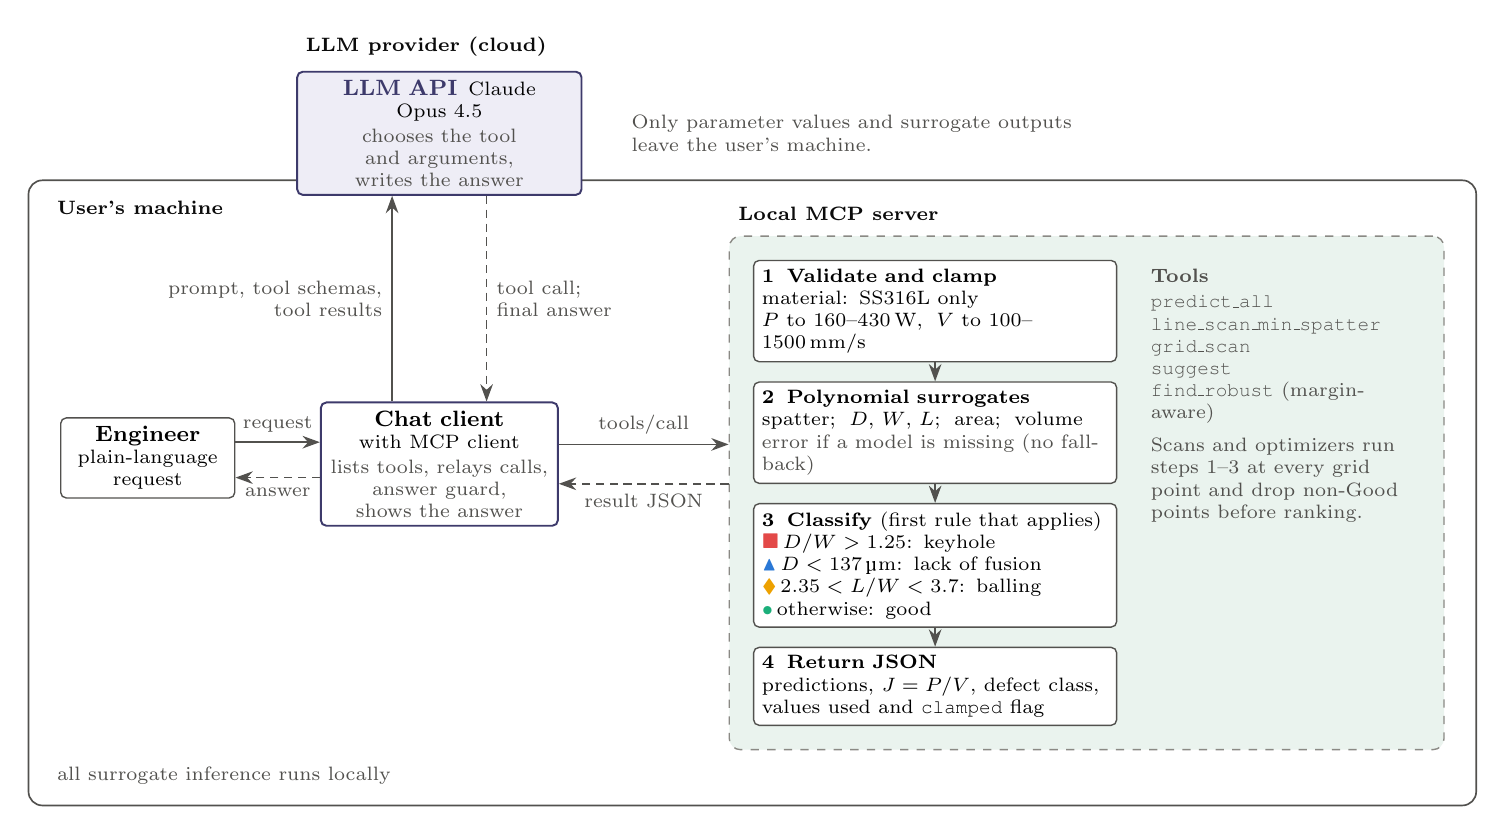
\begin{tikzpicture}
% ================= cloud: LLM provider (top)
\node[box, draw=agent, fill=agentbg, text width=34mm, anchor=north west, font=\scriptsize, line width=0.7pt] (llm) at (30mm,0) {%
\textbf{\footnotesize\textcolor{agent}{LLM API}}\enspace Claude Opus 4.5\\[1pt]{\color{ink2}chooses the tool and arguments,\\ writes the answer}};
\node[lab, anchor=south west, font=\scriptsize\bfseries, text=ink] at ($(llm.north west)+(0,0.6mm)$) {LLM provider (cloud)};

% ================= user's machine: engineer, chat client
\node[box, text width=20mm, anchor=north west, font=\scriptsize] (user) at (0,-44mm) {\textbf{\footnotesize Engineer}\\plain-language request};
\node[box, text width=28mm, anchor=north west, font=\scriptsize, draw=agent, line width=0.7pt] (client) at (33mm,-42mm) {%
\textbf{\footnotesize Chat client}\\with MCP client\\[1pt]{\color{ink2}lists tools, relays calls,\\answer guard, shows the answer}};
\draw[flow] ($(user.east)+(0,2mm)$) -- node[lab, above, font=\scriptsize]{request} ($(client.west|-user.east)+(0,2mm)$);
\draw[ret]  ($(client.west|-user.east)+(0,-2.5mm)$) -- node[lab, below, font=\scriptsize]{answer} ($(user.east)+(0,-2.5mm)$);

% ================= local MCP server pipeline
\node[box, anchor=north west, text width=44mm, align=left, font=\scriptsize] (s1) at (88mm,-24mm) {%
\textbf{1\enspace Validate and clamp}\\
material: SS316L only\\
$P$ to 160--430\,W,\; $V$ to 100--1500\,mm/s};
\node[box, anchor=north west, text width=44mm, align=left, font=\scriptsize] (s2) at ($(s1.south west)+(0,-2.4mm)$) {%
\textbf{2\enspace Polynomial surrogates}\\
spatter;\; $D$, $W$, $L$;\; area;\; volume\\
{\color{ink2}error if a model is missing (no fallback)}};
\node[box, anchor=north west, text width=44mm, align=left, font=\scriptsize] (s3) at ($(s2.south west)+(0,-2.4mm)$) {%
\textbf{3\enspace Classify} (first rule that applies)\\
\textcolor{kh}{$\blacksquare$}\,$D/W > 1.25$: keyhole\\
\textcolor{lof}{$\blacktriangle$}\,$D < 137$\,\textmu m: lack of fusion\\
\textcolor{ball}{$\blacklozenge$}\,$2.35 < L/W < 3.7$: balling\\
\textcolor{good}{$\bullet$}\,otherwise: good};
\node[box, anchor=north west, text width=44mm, align=left, font=\scriptsize] (s4) at ($(s3.south west)+(0,-2.4mm)$) {%
\textbf{4\enspace Return JSON}\\
predictions, $J = P/V$, defect class,\\values used and \texttt{clamped} flag};
\draw[flow] (s1) -- (s2); \draw[flow] (s2) -- (s3); \draw[flow] (s3) -- (s4);
\node[lab, anchor=north west, align=left, font=\scriptsize, text width=33mm] (tl) at ($(s1.north east)+(3mm,0)$) {%
\textbf{\scriptsize Tools}\\[1pt]
\texttt{predict\_all}\\\texttt{line\_scan\_min\_spatter}\\\texttt{grid\_scan}\\\texttt{suggest}\\\texttt{find\_robust} (margin-aware)\\[4pt]
Scans and optimizers run steps 1--3 at every grid point and drop non-Good points before ranking.};
\begin{scope}[on background layer]
  \node[region, fill=serverbg, fit=(s1)(s2)(s3)(s4)(tl), inner sep=3mm] (srv) {};
  \node[draw=ink2, line width=0.6pt, rounded corners=5pt, fit=(user)(client)(srv), inner xsep=4mm, inner ysep=7mm] (machine) {};
\end{scope}
\node[lab, anchor=south west, font=\scriptsize\bfseries, text=ink] at ($(srv.north west)+(0,0.6mm)$) {Local MCP server};
\node[lab, anchor=north west, font=\scriptsize\bfseries, text=ink] at ($(machine.north west)+(2.5mm,-1.5mm)$) {User's machine};
\node[lab, anchor=south west, font=\scriptsize, text=ink2] at ($(machine.south west)+(2.5mm,1.5mm)$) {all surrogate inference runs locally};

% ================= flows
\coordinate (cu) at ($(client.north)+(-6mm,0)$);
\coordinate (cd) at ($(client.north)+(6mm,0)$);
\draw[flow] (cu) -- node[lab, left, font=\scriptsize, align=right]{prompt, tool schemas,\\tool results} (cu|-llm.south);
\draw[ret]  (cd|-llm.south) -- node[lab, right, font=\scriptsize, align=left]{tool call;\\final answer} (cd);
\draw[flow] ($(client.east)+(0,2.5mm)$) -- node[lab, above, font=\scriptsize]{tools/call} ($(srv.west|-client.east)+(0,2.5mm)$);
\draw[ret]  ($(srv.west|-client.east)+(0,-2.5mm)$) -- node[lab, below, font=\scriptsize]{result JSON} ($(client.east)+(0,-2.5mm)$);
\node[lab, font=\scriptsize, text=ink2, align=left, anchor=west] at ($(llm.east)+(5mm,0)$) {Only parameter values and surrogate outputs\\leave the user's machine.};
\end{tikzpicture}
\end{document}
